\begin{columns}[totalwidth=.85\linewidth]
    \column{\textwidth}
    \vspace{-10mm}
        \begin{itembox}[l]{Initial Structure Generation\cite{sasaki}}
            \begin{enumerate}
                % \item \alert{実空間}で8-Chain Model から初期構造を作成。
                \item 8-Chain Model is used as starting structure in \alert{Real space}.
                    \begin{itemize}
                        \normalsize
                        % \item 所望の分岐数に\alert{ランダム}に選択した\alert{結合を除去}
                        \item Randomly selected edge is removed until desired functionality.
                        % \item 除去したジオメトリーに対応した\alert{トポロジーモデル}
                        \item Topological model is generated. 
                    \end{itemize}
                % \item トポロジー空間でランダム性の導入
                \item Randomness is introduced in \alert{topological space}.
                    \begin{itemize}
                        \normalsize
                        % \item \alert{エッジ交換}して、ノードごとにランダムな接続性を導入
                        \item By \alert{edge exchange}, random connectivity is introduced for each node.
                    \end{itemize}	
                % \item 対応する\alert{実空間でのネットワーク初期構造}を作成
                \item Corresponding real space structure is generated as initial model.
                % \item \alert{ストランド長がホモポリマーに対応}するように多重度設定
                \item According to e2e distance of strand, system size and multiplicity are set.
            \end{enumerate}

            \vspace{-1mm}
            \begin{columns}[T, onlytextwidth]
                \column{.33\linewidth}
                    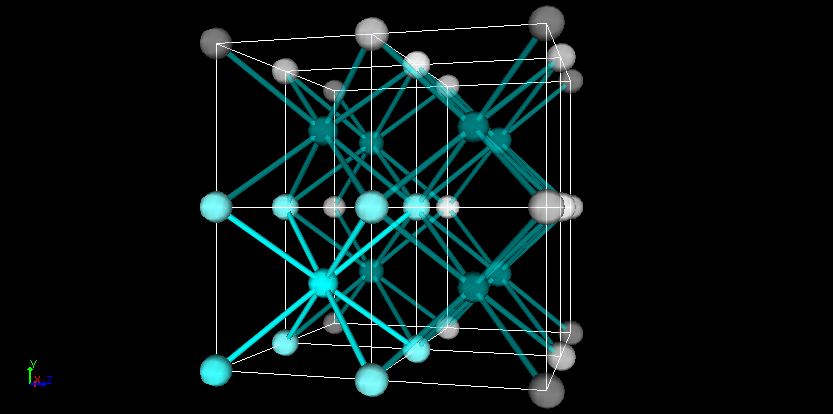
\includegraphics[width=\textwidth]{8_per.png}
                \column{.33\linewidth}
                    \vspace{-5mm}
                    \begin{center}
                        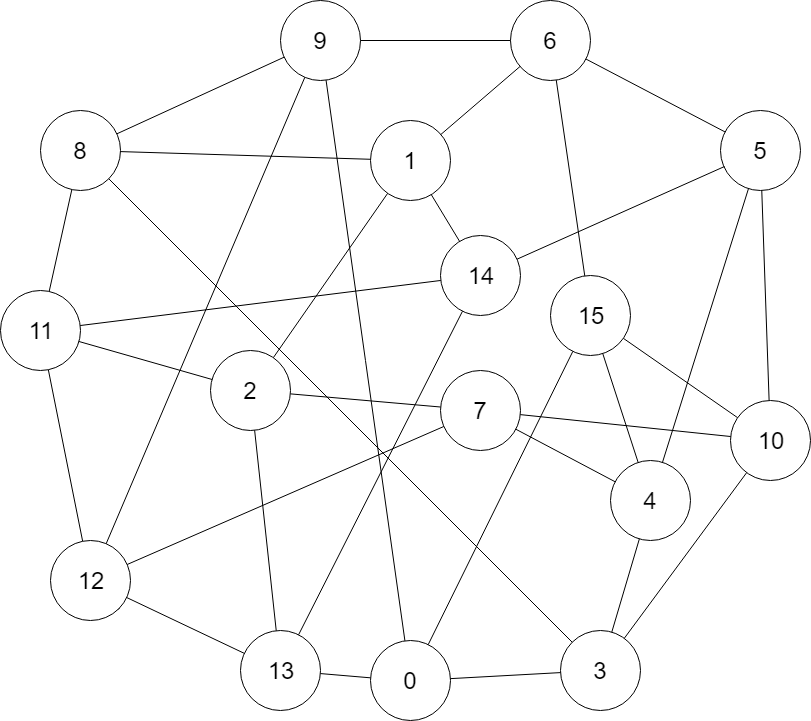
\includegraphics[width=.6\textwidth]{Network.png}
                    \end{center}
                \column{.33\linewidth}
                    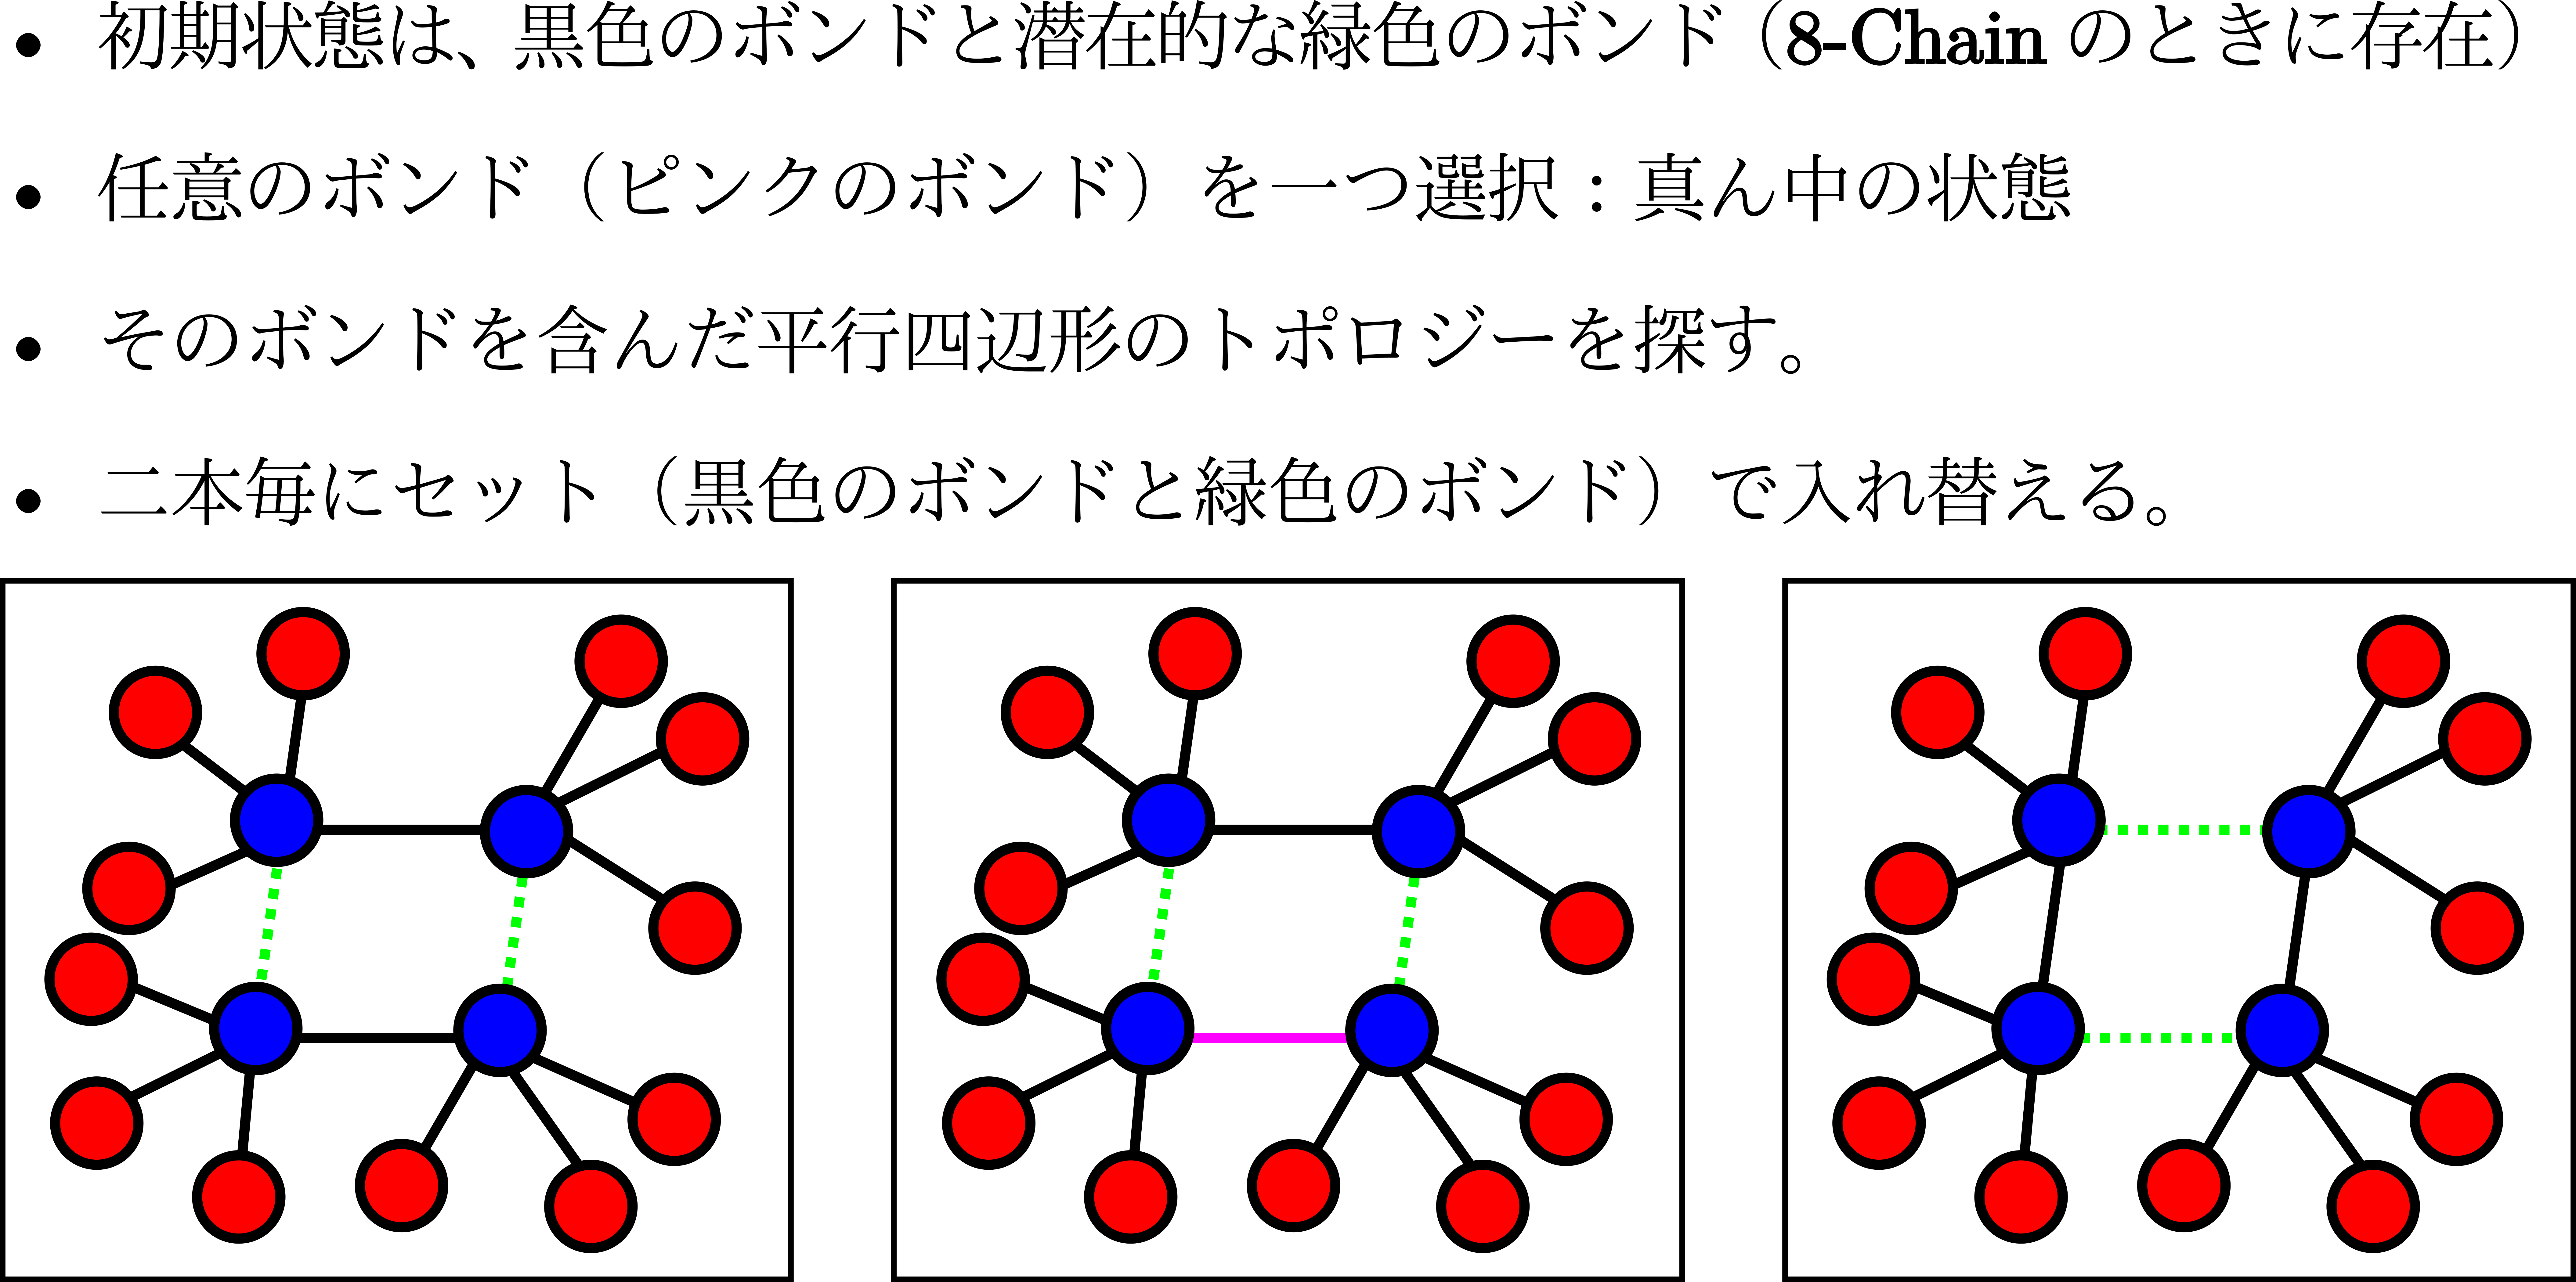
\includegraphics[width=\textwidth]{bond_exchg.png}
            \end{columns}
        \end{itembox}

        \begin{itembox}[l]{MD Simulation Conditions}
            \begin{enumerate}
                \item Phantom Chain
                    \begin{itemize}
                        \normalsize
                        \item No Excluded Volume is set (no segmental interaction).
                        \item "Force Cap LJ" is set as Angle Potential to enumerate KG Chain length.
                        \item Harmonic bond(k=1000)
                    \end{itemize}
                \item Length and Multiplicity
                    \begin{itemize}
                        \normalsize
                        \item Strand length in Initial Structure is set according to e2e distance of strand.
                        \item To set the system density ($\rho = 0.85$), network is multiplied as IPN.
                    \end{itemize}	
            \end{enumerate}
        \end{itembox}
\end{columns}